\section{Computer Experiments} \label{ch:computer_experiments}
This section describes the setup and configuration of the computational experiments conducted in this study, and the accompanied results. Two types of statistical models, \acrshort{convlstm} and \acrshort{ar}-model are trained and evaluated on an unseen portion of the dataset. 

\subsection{Framework, Structure and Implementation} \label{sec:structure_and_implementations} \label{sec:framework}
The numerical methods used in this study are described in Chapter \ref{ch:num_methods}. The code is available on GitHub in the project repository named ``MS'' on \href{https://github.com/hannasv/MS}{https://github.com/hannasv/MS}. Instructions for downloading 
reanalysis (ERA5) data using python is provided. 
The dataset is not published because of a licences on the \acrshort{msg} data. 
%The repository contains everything need to reproduce the results in this study.
%The experiments are conducted in notebooks and the developed modules are stored in the package ``sciclouds''. Descriptions on how to acquire the data (scripts if possible) and project environment is provided to simplify the process.

The code is developed in Python 3.7, a popular language for scientific software development. The source code is stored in the package \textit{sciclouds}, made available on Github through the project repository. Developed modules draw inspiration from the structure of \textit{scikit-learn} (\cite{sklearn_api}).
%and the \textit{keras-tuner} (\cite{chollet2015kerastuner}). 
%The \acrshort{convlstm} is implemented %in \textit{keras} (\cite{chollet2015keras})
%using \textit{tensorflow v 2.0} . %The \textit{keras-tuner} is used to automize the hyperparameter search (\cite{chollet2015kerastuner}). 
The \acrshort{convlstm} is implemented using Tensorflow's keras API (\cite{tensorflow2015}) which simplifies many aspects of building and executing machine learning models. To utilize the analytical solution the \acrshort{ar}-models are trained and evaluated using self implemented modules.
%The \acrshort{ar}-models are trained and evaluated using self implemented modules. The idea was to utilize the analytical solution of the least squares problem. 
%Many regression modules provide a numerical solution, not the analytical. 
The python package ``sclouds'' provides a self implemented version of \acrshort{ar}-models, using the analytical solution to the least squares problem derived in Section \ref{sec:ARmodels}.

Visualizations are generated using \textit{Matplotlib} (\cite{matplotlib}),  \textit{Seaborn} (\cite{seaborn}) and maps using the package \textit{Cartopy} (\cite{Cartopy}). Other illustrations are developed using TIkZ, a language used for producing technical illustrations within the environment of LaTeX.

The package versions are documented in the \textit{requirements.txt} and the project environment called ``sciclouds'' is ready for installation. This is a conda environment, the yaml-file lists the Python packages and requirements necessary for running this code. Below you find the code example for cloning the project and installing the environment.

% Included in the readme file on github. 
\begin{verbatim}
git clone https://github.com/hannasv/MS.git
cd MS
conda env create -f environment.yml
conda activate sciclouds
python setup.py install # installing package from source
\end{verbatim}

Supplementary material for remapping satellite data and filtering masks is available in the supplementary repository \href{https://github.com/hannasv/MS-suppl}{https://github.com/hannasv/MS-suppl}. %To make use of all the functionality available trought ``MS'', the supplementary repository needs to be cloned in the same directory.
The filters are generated from within the environment of PyAEROCOM (\cite{pyaerocom}). 


%Complex computations will cause memory growth, dependant on how many intermediate computations it needs to store. This is the case for \acrshort{convlstm}. To speed up the development process the software is developed on a subset of \acrshort{ecc}. Small adjustments needs to be made, running experiments on the entire data. For instance threads deadlock when extracting large amounts of data. This is a precautionary measure to avoid overloading the system. \textbf{Possible to develop code to do Hyperparameter tuning based on }
%For a more detailed description please see the project repository described in Section \ref{sec:structure_and_implementations}.

\subsection{Hardware} \label{sec:hardware}
%How to deal with big datasets that will easily eat up you memory? ``Big data'' involve processing large amounts of data that does not fit into memory. Processing substantial amounts of data require expert knowledge about distributed systems and analysing for system bottlenecks.  %Although theoretically fascinating it remains to see if \acrshort{convlstm} provide a clear practical advantage over the autoregressive models.
%Conducting experiments on big datasets require external computational resources.  
The experiments described below, are conducted on a 
%This study had access to a 
DGX-2 system consisting of 16 NVIDIA Tesla V100 GPUs, each of 32Gb local memory and 1.5Tb shared memory. %The resources was available through the \acrfull{ex3} project hosted at Simula. 
%This study was awarded access to 1 GPU and 1024G part of the memory. 
The data is stored on a \acrfull{rdma} accessed over Infiniband. %\textit{The best choice of collective implementation depends upon the number and kind of \acrshort{gpu}s, and the network interconnect in the cluster.} 
The DGX-2 system is designed for a high level concurrency and scheduling workers competing for system resources.
%The hardware sets the limitations for efficiency of pipelines and training procedure. 
%\textit{NVIDIA V100 GPU -- The eX3 infrastructure includes a DGX-2 system consisting of 16 NVIDIA Tesla V100 GPUs, allowing simultaneous communication between all eight GPU pairs at 300 GBps through the 12 integrated NVSwitches. This gives a theoretical system-wide system bi-directional  bandwidth of 2.4 TBps. All GPUs have 32 GB of local memory (total of 512 GB) and share a 1.5 TB main memory. The total system has 81,920 CUDA cores, and 10,240 Tensor cores delivering 2 Petaflops of tensor performance. The peak performance in double precision is 125 Teraflops.}
%Working on such a monstrosity pose additional challenges related to porting existing code and virtual environments, developing and debugging code. To eventually end up with an%a achieved 
%acceptable level of efficiency and reliability. \textbf{må de siteres? (\cite{ex3docs} and \cite{ex3homepage}).} 
\begin{table}[ht]
    \centering
    \begin{tabular}{c|c}
        Device &  Type  \\ \hline
        GPU & Tesla V100-SXM3-32GB \\
        CPU & DualProcessor AMD Epyc7601 (SMT2) w/2TB ram and 4TB NVMe 
    \end{tabular}
    \caption{Hardware specifications for the environment used on \acrshort{ex3}. The operating system is Ubuntu 18.04.4.}
    \label{tab:hardware_ex3}
\end{table}
%\textbf{TS: Mye av teksten frem til dette punktet egner seg egentlig bedre i et Appendix}
%TS: Mye av teksten frem til dette punktet egner seg egentlig bedre i et Appendix
\subsection{Model Setup and Evaluation}
The following sections contain the configurations of the models compiled for this study. A configuration is a set of parameters set prior to training. These are often referred to as hyperparameters, as mentioned in Section \ref{sec:artificial neural networks}.

%A model is compiled based on a choice of hyperparameters. It is a set of decisions made prior to training, as mentioned in Section \ref{sec:artificial neural networks}.
In the search for the best model configuration, different combinations of hyperparameters are evaluated based on a metric. % mention why you chose M;A;E?
This study evaluate models based on \acrfull{mae}, see Section \ref{sec:metrics} for more details.

For the more complex \acrshort{dl}-models, the choice of architecture (model configuration) can easily overload the system memory resources. Therefore the tuning of \acrshort{convlstm}-models was done manually. There is a mind-boggling amount of choices for hyperparameters, the initial configuration used in the conducted experiments for this project draw inspiration from this paper by \citeauthor{SunAirLSTM} (\citeyear{SunAirLSTM}).
The models are described in Section \ref{sec:related_work}.
The \acrshort{ar}-models follow another strategy. For this study the simplest models was trained first, followed by a gradual increase in complexity.
%This could have been done using spaced sampling, attempting lags of 1, 2, 5, 10. The result becomes the same, however for large model there might be some time to save.

%it follows the principal of starting with the simplest model possible and increasing the complexity from there. 
%Stopping at architectures where increased complexity don't increase the performance? Know stategies are using spaced sampling, attempting lags of 1, 2, 5, 10. The second is naturally to further investigate regons of lags showing the most promise. 
%on a similar problem, air quality forecasting problem was executed. \citepaper{chollet2015kerastuner} provide suitable software for the automatic hyperparameter tuning. 
%\textbf{Man kjører eksperimenter på mange modeller ved å bruke traning og validations dataset. The choice of model is based on this data basis and then it performance is tested on the test dataset.} 
\subsection{Training, validation and test split}
Gradient methods are at the heart of every machine 
learning algorithms. This type of optimization is based on the principle that the model is continuously evaluated against the validation dataset and weights are adjusted to reduce the loss. This raises the need for two datasets during training. The \acrshort{ar}-models are computed based on an analytical solution and have no need for the extra data set. 

Based on the assumption that the most resent partition is representative for the near future, both models were tested on 2014 to 2018. The \acrshort{ar}-model is trained on the period 2004 to 2013, while the \acrshort{convlstm} is trained on  2004 to 2011 and validated on 2012 to 2013.

Other notable differences in the input data is related to handling missing values.  
%Missing data arise from failed retrivals. Consequently entire grids are missing and not individual pixels. 
The \acrshort{ar}-models use shorter sequences, and samples containing missing values are simply removed. The \acrshort{convlstm}-model utilize longer sequences, and missing values are replaced by the out-of-sample value, $c=1.5$. 

%The test period was chosen based on the assumption that the latest period is most representative for the climate in the near future. The handling \textbf{(nytt ord)} of gaps, provide an additional difference to the datasets used as input for the \acrshort{ar} and the \acrshort{convlstm}-models. The order of the \acrshort{ar}-model determines the length of the training sequence. All samples with gaps in the requested sequence are disregarded causing a reduction in the data basis for a model of a particular order, determined by the number of lags. For the \acrshort{convlstm} these gaps are filled with an out-of-sample value, $c=1.5$. 
\subsection{Autoregressive models (AR)}
In this study a \acrshort{ar}-model is composed of 13041 individual regression models, one for each grid box. Four hyperparameters are possible to tune, \textit{feature scaling of the predictors}, the \textit{inclusion of bias}, \textit{number of lags} and a \textit{potential inclusion of environmental variables}. Varying combinations of these parameters results in the set of models trained in this study. More theoretical details can be found in Section \ref{sec:ARmodels}. 

\subsubsection{Feature Scaling} \label{sec:scaling_predictors}
Feature scaling is used to standardize the predictor variables.
\begin{equation} \label{eq:scaling_data}
    \mathbf{x} = \frac{\mathbf{x} - \bar{\mathbf{x}}}{\text{STD}(\mathbf{x})}
\end{equation}
The transformation is computed by applying Equation \eqref{eq:scaling_data} to the predictors, represented by $\mathbf{x}$. $\bar{\mathbf{x}}$ is its average and STD is its standard deviation. The resulting data has a reshaped distribution resembling a standard normal distribution, with zero mean and unit variance. This offers an additional benefit of increased numerical stability. %When applied the predictors is transformed according to the following Equation \ref{eq:scaling_data}. 
%The feature scaling is applied after the partitioning into training and test portions. 

It is important to perform the transformation after the data is split into training and test. The mean and standard deviation should be computed based on the training set and applied to both sets. The model is trained to find relations in transformed data. Consequently the test data need to be transformed before the model can be evaluated. 

The partitioning of datasets prior to the transformation is necessary to avoid a information leak between the test data and the trained model. If it was done differently it would result in an unrepresentative measure on performance.

 

%\subsubsection{Transforming target} \label{sec:transforming_target}
%A trick to avoid predicting unphysical values is fitting against a transformed target. In this study, the target, \acrfull{cfc} ranges from 0 to 1. By applying the inverse sigmoid transformation, see Equation \eqref{eq:inv_sigmoid} the target takes values from the entire real axis $(-\infty, \infty)$. 
%\begin{equation} \label{eq:inv_sigmoid}
%   \sigma^{-1} \left( x \right) = ln \left(\frac{x}{x - 1 + \epsilon} \right)
%\end{equation}
%In the above equation $\epsilon = 10^{-300}$ is added as a precaution for when $x=1$ and division by zero would occur. This would result in the non-numerical value, $-\infty$. The inverse transformation of this is ordinary sigmoid, see Equation \eqref{eq:sigmoid}. By applying this equation values return to the range between 0 and 1, alleviating predictions of out-of-sample values. The sigmoid function is described in Section \ref{sec:artificial neural networks} in the context of its abilities as an activation function in machine learning models and its graph is displayed in Figure \ref{fig:activation_function_example}.

\subsubsection{Lags and Environmental variables}
The dataset prepared for a particular model is determined by the number of lags and the inclusions of environmental variables (temperature, surface pressure, relative and specific humidity). This controls a models the number of degrees of freedom. All models are trained either on the full set of environmental variables or none of them. They never appear in isolation. 

Lags describe the number of previous timesteps of \acrshort{cfc} included as a predictor. For example, if the lag is three, $L=3$, then the \acrshort{cfc} is predicted based on the cloud cover for the previous three hours. To clear any confusion, all time steps back three hours are included.

%%%%%%%%%%%%%%%%%%%%%%%%%%%%%%%%%%%%%%%%%%%%% TRUDE RETTET OVER HER

\subsubsection{Experimental setup} \label{sec:experiments_ar}
The naming conventions for the \acrshort{ar}-models used in this study $AR_{TB_L}$ or $TR_{TB_L}$. $AR$ or $TR$ describe whether the environmental variables are included in the dataset of not. $TR$ is short for traditional and represent the case when environmental variables is omitted. \acrshort{ar} represent the opposite, their inclusion. B represent bias, T symbolize that scaling predictors is applied and $L_x$ reveals the number of lags, represented with $x$.  

%This description elaborated in Table \ref{tab:ar_model_config}.
To ease the understanding of the naming convention used, Table \ref{tab:ar_model_config} provide four examples. Applying the following convention, $\times$ denoted not applied, \checked denotes applied.
The hyperparameters bias and transformation of the predictors is mutually exclusive. Applying both have no benefits as the transformation could cancel the effect of the bias when subtracting the mean. 
\begin{table}[h]
    \centering
    %\resizebox{\textwidth}{!}{%
    \begin{tabular}{ccccc}
 & \textbf{Feature Scaling} & \textbf{Lag} &\textbf{ Environmental Variables} & \textbf{Bias} \\ \hline
    \multicolumn{1}{c}{\textbf{$TR_{B_1}$}} & $\times$  & 1 & $\times$ & \checked   \\ \hline
    \multicolumn{1}{c}{\textbf{$AR_{B_0}$}} & $\times$  & 0 & \checked  & \checked  \\ \hline
    \multicolumn{1}{c}{\textbf{$AR_{T_1}$}} & \checked  & 1 & \times & \times  \\ \hline
    \multicolumn{1}{c}{\textbf{$AR_{B_4}$}} & $\times$  & 4 & \checked & \checked  \\ \hline
    \end{tabular}%
    %}
    \caption{Example configuration of \acrshort{ar}-models, where $\times$ denoted not applied, \checked denotes applied.}
    \label{tab:ar_model_config}
\end{table}

\subsubsection{Evaluation}
The models are all evaluated using \acrfull{mae} and the \acrshort{ar}-models are optimized to fit the next timestep, not longer sequences. Figure \ref{fig:heatmap_ar_models} show the performance of all \acrshort{ar}-models included in this study, varying the number of lags on the first axis and the other hyperparameters on the second axis. The score is computed computed by using Equation \eqref{eq:mae}, and putting the parameters $m = 81$, $n=161$ and $k=43824$. 
\begin{figure}
    \centering
    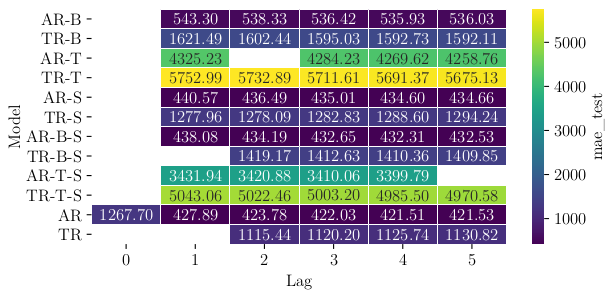
\includegraphics{python_figs/heat_ar_model_mae_test_score.png}
    \caption{Heatmap showing the area averaged test \acrshort{mae} for all the \acrshort{ar}-models included in this work. }
    \label{fig:heatmap_ar_models}
\end{figure}

With the exception of the $AR-T$-configuration, most models increase most rapidly in performance when adding the first lag. The performance continue to increase for larger numbers of lags, but at a much slower rate. This shows that the cloud cover at previous timesteps is a useful predictor. The largest variations in performance is caused by varying configurations of $AR$, $B$, $T$ and $TR$. 

%%%%%%%%%%%%%%%%%%%%% Ta for deg alle variablene. 
The models employing, $T$ have the lowest score. A grid \acrshort{mae} of roughly $0.5$ is quite a lot when the target varies in the range from 0 to 1. The inclusion of a bias, in combination with $AR$ improves the performance, for $TR$ it has the opposite effect and decrease the performance. In conclusion, $T$ is not a setting for the cloud forecasting problem.


The $TR$-configuration perform a lot better than $T$, and the set of models lie close to $0.14$. Since $AR$ outperforms $TR$ for all configurations, except for $T$. This indicates that the environmental variables provide useful information.

The skill of the best model, $AR-B-L_5$, is $0.04901$, which is great.
% This is to great, the model overfitted and is unable to generalize
Showing that there is enough information in the set of environmental variables and previous cloud cover to predict one hour into the future.
\subsubsection{Weights in $\mathbf{AR-B-L_5}$}
%%%%%%%%%%%%%%%%%%%% TEXT ON WEIGHTS 
\begin{figure}
    \centering
    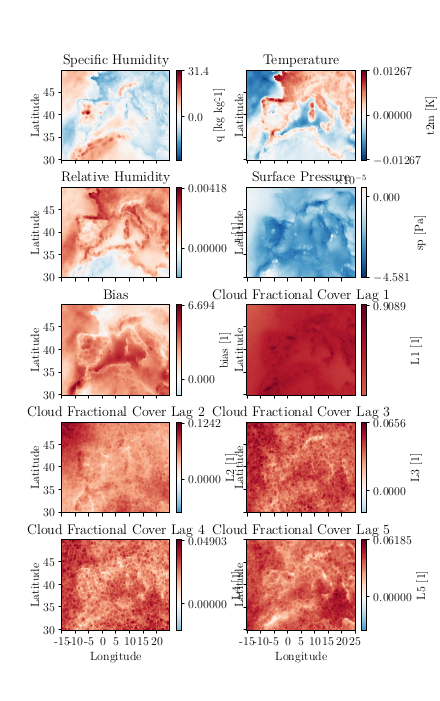
\includegraphics[scale=0.9]{python_figs/weights_AR-B-L5_best_ar_model.png}
    \caption{The weights of the $AR-B-L_5$-model.}
    \label{fig:weights_best_model}
\end{figure}
Figure \ref{fig:weights_best_model} shows the weights in $AR-B-L5$. The colorbars are different for all subplots, but the colors are consistent. Red being positive and blue is negative. The \acrshort{ar}-model is a weighted sum over all the variables. Negative input values are unphysical, with the exception of $r$, it is not present, as documented in Section \ref{sec:all_stats}. In the case of relative humidity, $r$ they are rarely present, but exist, and the minimum values is $-6.6505$. 

Surface pressure is negative for the entire grid. Higher pressure produce larger reductions in cloud cover. This is in agreement with the cloud physics described in Section X, stating that in areas of high pressure are assosiated with descending airmasses and that does not produce clouds. 

%\textbf{The follwowing statement is true for the remaining variables}
For the other variables, positive values contribute to cloud formation and negative values to dissipation.

By studying the weights of the five hours of previous timesteps its clear that they all contribute in producing cloud cover, there $L_1$ have the highest weights. They are close to one for the entire grid. The minor change for increasing number of lags, shown in Figure \ref{fig:heatmap_ar_models}, can be attributed to the small magnitude of the weights of other lags. 
%\textbf{This explains the copying effect seen in the sequence plotted.}

The behavior of relative and specific humidity is puzzling, they exhibit the approximately opposite pattern. North Africa has one sign, and Europe has another. In most regions where relative humidity produce clouds, specific humidity reduce it cloud cover. In regions over Spain the same appears to be going on with temperature and specific humidity. 

\clearpage

\subsection{Convolutional LSTM (ConvLSTM)}
The formulation of the air quality forecasting problem presented by \citeauthor{SunAirLSTM} is similar to the formulation of the cloud fractional cover forecasting problem presented in this study. 
%The machine learning experimental setup is adopted from the paper \citepaper{SunAirLSTM}.
% Endrer på arkitekturen - denne bruker -train - validation - test, en hvis prosentandel a
This study adopts the machine learning setup in \citepaper{SunAirLSTM}. Manually tuning of the models are applied to avoid a breakdown of the computer caused by to many parameters. When building \acrshort{convlstm} networks, the list of tunable parameters is extensive. In this work a subset of them is tuned and the rest is kept constant.

The following section describe the tuned hyperparameters, batch size, sequence length, number of hidden state and the dimensions of the kernel (\textbf{med fnutter?}). The dataset is partitioned into subsets called batches. The batch size is the number of sequences a weight update is based on. Epochs describes the number of times the model loops over the entire dataset, \textbf{denne varierer du jo strengt talt ikke}. The sequence length is the number of timestamps a model is optimized to learn to predict. The number of hidden states it the number of filters it learns in each layer, see Section \ref{sec:convolutional neural network} for a detailed description of hidden states. 
The filter\textbf{eller kernel} size determines the number of neighbors influencing an activation. Using kernel 1x1 results in the state-to-state transitions similar to \acrshort{ar}-models by removing interactions between adjacent pixels. A more detailed description on these parameters is provided in Sections \ref{sec:convolutional neural network} to \ref{sec:convolutional_lstm}. 

This section describe the hyperparameters kept constant. Between each \acrshort{convlstm}-layer there is a \acrfull{batchnorm}-layer, implemented using default settings. This was first used by \citepaper{ioffe2015batch} convolutional neural network and it showed three benefits, the network was less sensitive to the weight initialization, learning rate and it didn't need dropout. Another hyperparameter, which randomly removing some of the trained weights to prevent overfitting. This is computationally expensive, disabling dropout accelerate the training process.
``Padding same'' is applied to all \acrshort{convlstm}-layer, to make sure the input and output dimensions are the same, see Section \ref{sec:padding}. The model returns a sequence and the input sequences are not shuffled. The output filter and kernel size is one to concatenate all the previous hidden states to one without altering the output dimension. This is necessary to predict a sequence of cloud fractional covers. 

The weights were initialized based on the scheme ``LeCun uniform''  (\cite{Lecun98efficientbackprop}). Callbacks such as %early stopping was impleme with patience \textbf{forgot to apply this when rerunning the models..} of 10 epochs and 
terminate on NaN's have been applied to avoid prolonged training time. The optimizer ADAM is used with the following settings, $\text{learning rate}=0.001$, $\text{beta1}=0.9$, $\text{beta2}=0.999$, $\text{epsilon}=1e-07$ (\cite{Kingma2015Adam:Optimization}). The default settings in Tensorflow use $\text{epsilon}=1e-08$. The loss function is \acrfull{mse}, and the models are evaluate based on \acrfull{mae}.
Both functions are described in more detail in Section \ref{sec:metrics}. %The main difference between these functions is that \acrshort{mse} penalize points further away. This has its advantages in training the model, but makes it more difficult to interpret the results. The squared numbers in the range 0 to 1 shrink.

\subsubsection{Experimental setup}
Models are given names based on an extension of the convention from \citepaper{precip_nowcasting}.
The batch size and sequence length is included and 
the resulting naming convention is  $ConvLSTM-B_{x}-SL_{y}-\text{hidden states}-filter$\times$filter$. Table \ref{tab:convlstm_config} provide a set of example configurations, here the square brackets list the number of hidden states in each of the layers, so if the bracket has three members the network have three layers. 

\begin{table}[hp]
    \centering
    \resizebox{\textwidth}{!}{%
    \begin{tabular}{ccccc}
     \textbf{ConvLSTM Model} & \textbf{Sequence Length} & \textbf{Batch Size} & \textbf{Hidden States} & \textbf{Kernels} \\ \hline
    $B_{10}-SL_{24}-16-3\times3-16-3\times3$ & 24 & 10 & [16, 16]   & [3, 3] \\ \hline
    $B_{10}-SL_{24}-32-1\times1-32-1\times1$ & 24 & 10 & [32, 32]  & [1, 1] \\ \hline
    $B_{10}-SL_{24}-32-3\times3-32-3\times3$ & 24 & 10 & [32, 32] & [3, 3] \\ \hline
    $B_{10}-SL_{24}-32-5\times5-32-5\times5$ & 24 & 10 & [32, 32] & [5, 5] \\ \hline
    $B_{10}-SL_{24}-8-3\times3-8-3\times3-8-3\times3$ & 24 & 10 & [8, 8, 8] & [3, 3, 3] \\ \hline
    $B_{5}-SL_{6}-32-3\times3-32-3\times3-32-3\times3$ & 6 & 5 & [32, 32, 32] & [3, 3, 3] \\ \hline
    \end{tabular}%
    }
    \caption{Examples of \acrshort{conv}-model names and their configurations.}
    \label{tab:convlstm_config}
\end{table}

\subsubsection{Evaluation}
\textbf{Tenk på om du vil ha en egen ligning for dette, den er fire dimensjonal ikke 3 som ar.}
The input volume of \acrshort{convlstm}-models are different from the \acrshort{ar}-model, and the axis ``batch'' and ``sequence length'' are merged 
The score is computed computed by using Equation \eqref{eq:mae}, and putting the parameters $m = 81$, $n=161$ and $k=43680$. Note that the $k$ value is a bit smaller than for \acrshort{ar}-models, this is caused by employing the ``drop remainder batch'' during training. 

\begin{figure}
    \centering
    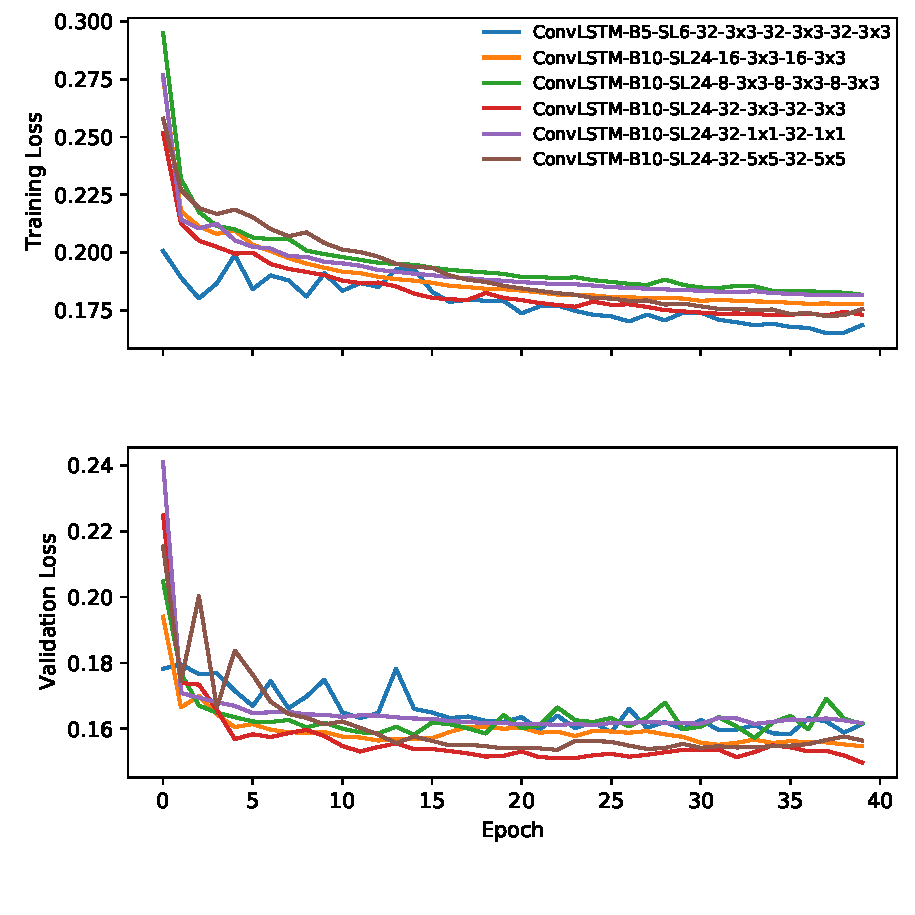
\includegraphics{python_figs/epoch_vs_loss.pdf}
    \caption{The loss of the trained model as a function of epochs.}
    \label{fig:convlstm_loss}
\end{figure}

Figure \ref{fig:convlstm_loss} shows the loss curves in the training process for all the compiled models in this study. As expected, they all ``learn'' the most rapidly in the beginning of the training process. This is shown in the figure as the abrupt drop i loss between epochs the first and second epoch. 

\textbf{Note that the training loss is higher than the validation loss since there is a higher number of samples in this set and the loss is not scaled by the number of samples.} 

%%%%%%%%%%%%%%%%%%%%%%%%% The copied dictionary is the result from tf.evaluate. 
\begin{table}[]
    \centering
    \resizebox{\textwidth}{!}{
    \begin{tabular}{c|lccc}
    \textbf{ConvLSTM Model} & \textbf{Train Loss} & \textbf{Val Loss} & \textbf{Test Loss} & \textbf{Num. Params.} \\ \hline 
    $B_{10}-SL_{24}-16-3\times3-16-3\times3$ & 0.1779 & 0.1547 & 0.1575 &  30 296\\ \hline
    % {"loss": 0.15752051770687103, "mean_squared_error": 0.15752056241035461, "r2_keras": 0.15506696701049805, "mean_absolute_error": 0.34570422768592834}

    $B_{10}-SL_{24}-32-1\times1-32-1\times1$ & 0.1817 & 0.1617 & 0.1649 & 13 464 \\ \hline
    % {"loss": 0.1649022251367569, "mean_squared_error": 0.1649022400379181, "r2_keras": 0.1159096509218216, "mean_absolute_error": 0.35085538029670715}
    \rowcolor{red!30}
    $B_{10}-SL_{24}-32-3\times3-32-3\times3$ & 0.1731 & 0.1497 & 0.1534 & 115 864 \\ \hline
    %{"loss": 0.15340088307857513, "mean_squared_error": 0.15340085327625275, "r2_keras": 0.17754235863685608, "mean_absolute_error": 0.33814743161201477}
    
    $B_{10}-SL_{24}-32-5\times5-32-5\times5$ & 0.1755 & 0.1564 & 0.1589 & 320 664 \\ \hline
    % {"loss": 0.15889282524585724, "mean_squared_error": 0.15889279544353485, "r2_keras": 0.147248774766922, "mean_absolute_error": 0.34079509973526}
    
    $B_{10}-SL_{24}-8-3\times3-8-3\times3-8-3\times3$ &  0.1817 & 0.1615 & 0.1634 & 12 920 \\ \hline
    % {"loss": 0.16335555911064148, "mean_squared_error": 0.16335561871528625, "r2_keras": 0.12448494136333466, "mean_absolute_error": 0.3477591276168823}
    
    $B_{5}-SL_{6}-32-3\times3-32-3\times3-32-3\times3$ & 0.1686 & 0.1615  & 0.1633 &  189 848 \\ \hline
    %{"loss": 0.1632702797651291, "mean_squared_error": 0.16327014565467834, "r2_keras": 0.09565786272287369, "mean_absolute_error": 0.3411720395088196}
    
      \end{tabular}
    }
    \caption{Results, metrics and number of parameters for the trained models. The best model \acrshort{convlstm}-model is highlighted in light blue. The loss presented is averaged over on batch, this is the keras default. Since its only used to chose the best model, there is no reason to upscale the numbers.}
    \label{tab:convlstmLoss}
\end{table}
From Figure \ref{fig:convlstm_loss} and Table \ref{tab:convlstmLoss} (highlighted in blue) its clear that the best performing \acrshort{convlstm}-model is the $ConvLSTM-B_{10}-SL_{24}-32-3\times3-32-3 \times3$. It has the lowest test and validation loss after 40 epochs. Anothe model $ConvLSTM-B_{5}-SL_{6}-32-3\times3-32-3 \times3-32-3 \times3$ had a better training loss. As you might have deduced based on the similarities in the names, the have similar architectures.
The last model has an additional layer, this may have allowed it to learn a better representation (or overfittet) on the training data presented, however the models are evaluated on unseen data and $ConvLSTM-B_{10}-SL_{24}-32-3\times3-32-3 \times3$ goes out winning.

In some cases reducing the spatiotemporal resolution will enable the model to learn even more (\cite{precip_nowcasting}). This is arguably not applicable for this task, since cloud cover has an average lifetime of one hour, as mentioned in Section \ref{sec:cloud_in_climate_system}. If applied it would most likely produce a significant loss of information.

\textbf{Overgangs}
Proving that this study has trained a \acrshort{convlstm}-model on a larger amount of data than earlier studies. Comparisons of input data to the works by \citeauthor{precip_nowcasting} (\citeyear{precip_nowcasting}) and \citeauthor{SunAirLSTM} (\citeyear{SunAirLSTM}), is done based on input volumes. The dimensions are flattened to generalize the comparison. \citepaper{precip_nowcasting} is trained on $1,629,600,000$ data points, \citepaper{SunAirLSTM} on $28,513,800$ and \acrshort{ecc} on $21,220,315,200$. Consequently, the models in this study is trained on more than 10 times the amount of data.

$ConvLSTM-B_{10}-SL_{24}-32-3\times3-32-3 \times3$-model architecture is shown in Figure \ref{fig:best_ml_architecture}. The model consist of three \acrshort{batchnorm} and  \acrshort{convlstm}-layer pairs. Both \acrshort{convlstm} layer have 32 hidden states and a $3\times 3$ kernel. The output layer has one hidden state and the kernel dimension of $1\times 1$. The input shape is $10\times24\times81\times161\times4$ and output $24\times81\times161\times1$. 
\begin{figure}
    \centering
    \begin{tikzpicture}[x={(1,0)},y={(0,1)},z={({cos(60)},{sin(60)})},
font=\sffamily\small,scale=1.9] % 1.7 passer bra på siden.

\tikzset{circle dotted/.style={dash pattern=on .05mm off 2mm,
                                         line cap=round}}

%
% comment these out if you want to see where the axes point to
% \draw[-latex] (0,0,0) -- (3,0,0) node[below]{$x$};
% \draw[-latex] (0,0,0) -- (0,3,0) node[left]{$y$};
% \draw[-latex] (0,0,0) -- (0,0,3) node[below]{$z$};
% a plane
\tikzset{pics/fake box/.style args={% #1=color, #2=x dimension, #3=y dimension, #4=z dimension
#1 with dimensions #2 and #3 and #4}{
code={
\draw[teal,ultra thin,fill=#1]  (0,0,0) coordinate(-front-bottom-left) to
++ (0,#3,0) coordinate(-front-top-right) --++
(#2,0,0) coordinate(-front-top-right) --++ (0,-#3,0) 
coordinate(-front-bottom-right) -- cycle;
\draw[teal,ultra thin,fill=#1] (0,#3,0)  --++ 
 (0,0,#4) coordinate(-back-top-left) --++ (#2,0,0) 
 coordinate(-back-top-right) --++ (0,0,-#4)  -- cycle;
\draw[teal,ultra thin,fill=#1!80!black] (#2,0,0) --++ (0,0,#4) coordinate(-back-bottom-right)
--++ (0,#3,0) --++ (0,0,-#4) -- cycle;
\path[teal,decorate,decoration={text effects along path,text={BATCH NORM}}] (#2/2,{3.4+(#3-2)/2},0) -- (#2/2,0,0);
}
}}
%3.0/1.5, 3.0/3.3, 3.0/5.0
\foreach \X / \Y in {3.0/1.3, 3.0/3., 3.0/4.6} 
%2.2,2.2,2.0
{
\draw pic (box1-\Y) at (\Y,-\X/2,0) {fake box=white!70!teal with dimensions 0.5 and {2*\X} and 1*\X};
}

%%%%%%%%%%%%%%%%%%%%%%%%%%%%%%%%%%%% 
\tikzset{pics/fake box/.style args={% #1=color, #2=x dimension, #3=y dimension, #4=z dimension
#1 with dimensions #2 and #3 and #4}{
code={
\draw[gray,ultra thin,fill=#1]  (0,0,0) coordinate(-front-bottom-left) to
++ (0,#3,0) coordinate(-front-top-right) --++
(#2,0,0) coordinate(-front-top-right) --++ (0,-#3,0) 
coordinate(-front-bottom-right) -- cycle;
\draw[gray,ultra thin,fill=#1] (0,#3,0)  --++ 
 (0,0,#4) coordinate(-back-top-left) --++ (#2,0,0) 
 coordinate(-back-top-right) --++ (0,0,-#4)  -- cycle;
\draw[gray,ultra thin,fill=#1!80!black] (#2,0,0) --++ (0,0,#4) coordinate(-back-bottom-right)
--++ (0,#3,0) --++ (0,0,-#4) -- cycle;
\path[gray,decorate,decoration={text effects along path,text={CONV LSTM}}] (#2/2,{3.4+(#3-2)/2},0) -- (#2/2,0,0);
}
}}

%%%%%%%%%%%%%%%%%%%%%%%%%%%%%%
\foreach \X / \Y in {3.0/1.6, 3.0/3.3, 3.0/4.9}
%2.2,2.2,2.0
{
\draw pic (box1-\Y) at (\Y,-\X/2,0) {fake box=white!70!gray with dimensions 0.5 and {2*\X} and 1*\X};
}

%\foreach \X/\Col in {0.0/red,0.2/green,0.4/cyan, 0.6/yellow, 6.8/blue} %{6.5/red,6.7/green,6.9/blue}
%{\draw[canvas is yz plane at x = \X, transform shape, draw = black, fill = \Col!50!white, opacity = 0.5] (0,0.5) rectangle (2,-1.5);}

%\draw[gray!60,thick] (-0.1,-0.1,-1.6) coordinate (1-1) -- (-0.1,-0.1,0.6) coordinate (1-2) -- (-0.1, 2.,0.6) coordinate (1-3) -- (-0.1, 2.1,-1.6) coordinate (1-4) -- cycle;
%\draw[gray!60,thick] (0.8,-0.1,-1.6) coordinate (2-1) -- (0.8,-0.1,0.6) coordinate (2-2) -- (0.8, 2.,0.6) coordinate (2-3) -- (0.8,2.1,-1.6) coordinate (2-4) -- cycle;

%%%%%%%%%%%%%%%%%%%%%%%%%%%%%%%%%%%% 
\tikzset{pics/fake box/.style args={% #1=color, #2=x dimension, #3=y dimension, #4=z dimension
#1 with dimensions #2 and #3 and #4}{
code={
\draw[gray,ultra thin,fill=#1]  (0,0,0) coordinate(-front-bottom-left) to
++ (0,#3,0) coordinate(-front-top-right) --++
(#2,0,0) coordinate(-front-top-right) --++ (0,-#3,0) 
coordinate(-front-bottom-right) -- cycle;
\draw[gray,ultra thin,fill=#1] (0,#3,0)  --++ 
 (0,0,#4) coordinate(-back-top-left) --++ (#2,0,0) 
 coordinate(-back-top-right) --++ (0,0,-#4)  -- cycle;
\draw[gray,ultra thin,fill=#1!80!black] (#2,0,0) --++ (0,0,#4) coordinate(-back-bottom-right)
--++ (0,#3,0) --++ (0,0,-#4) -- cycle;
\path[gray,decorate,decoration={text effects along path,text={INPUT}}] (#2/2,{2.4+(#3-2)/2},0) -- (#2/2,0,0);
}
}}

%%%%%%%%%%%%%%%%%%%%%%%%%%%%%%
\foreach \X / \Y in {3.0/-1.0}
%2.2,2.2,2.0
{
\draw pic (box1-\Y) at (\Y,-\X/2,0) {fake box=white!70!green with dimensions 2.5 and {2*\X} and 1*\X};
}

\tikzset{pics/fake box/.style args={% #1=color, #2=x dimension, #3=y dimension, #4=z dimension
#1 with dimensions #2 and #3 and #4}{
code={
\draw[gray,ultra thin,fill=#1]  (0,0,0) coordinate(-front-bottom-left) to
++ (0,#3,0) coordinate(-front-top-right) --++
(#2,0,0) coordinate(-front-top-right) --++ (0,-#3,0) 
coordinate(-front-bottom-right) -- cycle;
\draw[gray,ultra thin,fill=#1] (0,#3,0)  --++ 
 (0,0,#4) coordinate(-back-top-left) --++ (#2,0,0) 
 coordinate(-back-top-right) --++ (0,0,-#4)  -- cycle;
\draw[gray,ultra thin,fill=#1!80!black] (#2,0,0) --++ (0,0,#4) coordinate(-back-bottom-right)
--++ (0,#3,0) --++ (0,0,-#4) -- cycle;
\path[gray,decorate,decoration={text effects along path,text={OUTPUT}}] (#2/2,{2.6+(#3-2)/2},0) -- (#2/2,0,0);
}
}}

\foreach \X / \Y in {3.0/6.1}
%2.2,2.2,2.0
{
\draw pic (box1-\Y) at (\Y,-\X/2,0) {fake box=white!70!blue with dimensions 1.0 and {2*\X} and 1*\X};
}

%\foreach \X in {4,1,3}
%{\draw[gray!60,thick] (1-\X) -- (2-\X);}

\node[draw,single arrow, orange,fill=orange!30] at (0.8, 0.5,0) {BATCH};
\node[draw,single arrow, orange,fill=orange!30] at (2.4, 0.5,0) {$3\times 3$};
\node[draw,single arrow, orange,fill=orange!30] at (4., 0.5,0) {$3\times 3$};
\node[draw,single arrow, orange,fill=orange!30] at (5.6, 0.5,0) {$1\times 1$};

%\begin{scope}[on background layer]
%\node[orange,thick,rounded corners,fill=orange!30,fit=(A1) (A3)]{};
%\node[gray,thick,rounded corners,fill=gray!10,fit=(B1) (B3)]{};
%\end{scope}

%\foreach \X in {1,2,3}
%{\draw[-latex] (A\X) -- (B2);}

\draw[thick](0.2, 3.3)node[scale=1.]{\small $10\times 24\times 81\times 161 \times 4 $};
\draw[thick](1.5, -2)node[scale=1.]{\small $10\times 24\times81\times 161 \times 32 $};
\draw[thick](3.8, 3.3)node[scale=1.]{\small $10\times 24\times 81\times 161 \times 32 $};
\draw[thick](5.0, -2)node[scale=1.]{\small $10\times 24\times 81\times 161 \times 1 $};
\draw[thick](6.6, 3.3)node[scale=1.]{\small $10\times 24\times 81\times 161 \times 1 $};
\end{tikzpicture}
    \caption{The architecture of the cloud cover forecasting model developed in this study. }
    \label{fig:best_ml_architecture}
\end{figure}
In Figure \ref{fig:best_ml_architecture} is illustrated as a green box. The full details of the 5-dimensional input volume is displayed in Figure \ref{fig:input_volume_conv_lstm}. The inputvolume is divided into batches, for this model, a batch consist of a 10 sequences. A sequence is a timeseries of 24 hours. Each hour is $81\time161\times4$-dimensional, consisting of grids the four environmental variables, temperature, surface pressure, relative and specific humidity. 

\begin{figure}
    \centering
    
\tikzset{every picture/.append style={scale=1.0}}
\begin{tikzpicture}[x={(1,0)},y={(0,1)}, z={({cos(60)},{sin(60)})},
font=\sffamily\small, scale=1.0]

\tikzset{pics/fake box/.style args={% #1=color, #2=x dimension, #3=y dimension, #4=z dimension
#1 with dimensions #2 and #3 and #4}{
code={
\draw[teal,ultra thin,fill=#1,opacity=0.25]  (0,0,0) coordinate(-front-bottom-left) to
++ (0,#3,0) coordinate(-front-top-right) --++
(#2,0,0) coordinate(-front-top-right) --++ (0,-#3,0) 
coordinate(-front-bottom-right) -- cycle;
\draw[teal,ultra thin,fill=#1, opacity=0.25] (0,#3,0)  --++ 
 (0,0,#4) coordinate(-back-top-left) --++ (#2,0,0) 
 coordinate(-back-top-right) --++ (0,0,-#4)  -- cycle;
\draw[teal,ultra thin,fill=#1!80!black, opacity=0.25] (#2,0,0) --++ (0,0,#4) coordinate(-back-bottom-right)
--++ (0,#3,0) --++ (0,0,-#4) -- cycle;
\path[teal,decorate,decoration={text effects along path,text={}}] (#2/2,{3.4+(#3-2)/2},0) -- (#2/2,0,0);
}
}}

%%%%%%%%%% Green box in the back symbolizing batches 
\foreach \X / \Y in {2.3/-1.5} {
\draw pic (box1-\Y) at (\Y,-\X/,0) {fake box=green with dimensions 14.6 and {2*\X} and 1*\X};
}


%%%%%%%%%%%%%%%%%%%%%%%%%%%%%% BLUE BOX
\foreach \X / \Y in {1.5/-1.0, 1.5/6} {
\draw pic (box1-\Y) at (\Y,-\X/,0) {fake box=white!25!cyan with dimensions 6.9 and {2*\X} and 1*\X};
}


%%%%%%%%%%%%%%%%%%%%%%%%%%%%%%% Weather data volume 1.
\foreach \X/\Col in {0.0/red, 0.2/green, 0.4/cyan, 0.6/yellow} %{6.5/red,6.7/green,6.9/blue}
{\draw[canvas is yz plane at x = \X, transform shape, draw = black, fill = \Col!50!white, opacity = 0.5] (0,0.5) rectangle (2,-1.5);}

%\draw[gray!60,thick] (-0.1,-0.1,-1.6) coordinate (1-1) -- (-0.1,-0.1,0.6) coordinate (1-2) -- (-0.1, 2.,0.6) coordinate (1-3) -- (-0.1, 2.1,-1.6) coordinate (1-4) -- cycle;

%\draw[gray!60,thick] (0.8,-0.1,-1.6) coordinate (2-1) -- (0.8,-0.1,0.6) coordinate (2-2) -- (0.8, 2.,0.6) coordinate (2-3) -- (0.8,2.1,-1.6) coordinate (2-4) -- cycle;

%\foreach \X in {4,1,3}{\draw[gray!60,thick] (1-\X) -- (2-\X);}

\tikzset{pics/fake box/.style args={% #1=color, #2=x dimension, #3=y dimension, #4=z dimension
#1 with dimensions #2 and #3 and #4}{
code={
\draw[teal,ultra thin]  (0,0,0) coordinate(-front-bottom-left) to
++ (0,#3,0) coordinate(-front-top-right) --++
(#2,0,0) coordinate(-front-top-right) --++ (0,-#3,0) 
coordinate(-front-bottom-right) -- cycle;
\draw[teal,ultra thin] (0,#3,0)  --++ 
 (0,0,#4) coordinate(-back-top-left) --++ (#2,0,0) 
 coordinate(-back-top-right) --++ (0,0,-#4)  -- cycle;
\draw[teal,ultra thin,fill=#1!80!black] (#2,0,0) --++ (0,0,#4) coordinate(-back-bottom-right)
--++ (0,#3,0) --++ (0,0,-#4) -- cycle;
\path[teal,decorate,decoration={text effects along path,text={}}] (#2/2,{3.4+(#3-2)/2},0) -- (#2/2,0,0);
}
}}

%%%%%%%%%%%%%%%%%%%%%%%%%%%%%%%%%%%%%%%%%%%%

%%%%%%%%%%%%%%%%%%%%%%%%%%%%%% BLUE BOX

\foreach \X/\Col in {2.0/red,2.2/green,2.4/cyan, 2.6/yellow} %{6.5/red,6.7/green,6.9/blue}
{\draw[canvas is yz plane at x = \X, transform shape, draw = black, fill = \Col!50!white, opacity = 0.5] (0,0.5) rectangle (2,-1.5);}

\foreach \X/\Col in {5.0/red,5.2/green,5.4/cyan, 5.6/yellow} %{6.5/red,6.7/green,6.9/blue}
{\draw[canvas is yz plane at x = \X, transform shape, draw = black, fill = \Col!50!white, opacity = 0.5] (0,0.5) rectangle (2,-1.5);}

%%%%%%%%%%%%%%% Second bow
\foreach \X/\Col in {7.0/red,7.2/green,7.4/cyan, 7.6/yellow} %{6.5/red,6.7/green,6.9/blue}
{\draw[canvas is yz plane at x = \X, transform shape, draw = black, fill = \Col!50!white, opacity = 0.5] (0,0.5) rectangle (2,-1.5);}

\foreach \X/\Col in {9.0/red,9.2/green,9.4/cyan, 9.6/yellow} %{6.5/red,6.7/green,6.9/blue}
{\draw[canvas is yz plane at x = \X, transform shape, draw = black, fill = \Col!50!white, opacity = 0.5] (0,0.5) rectangle (2,-1.5);}

\foreach \X/\Col in {12.0/red,12.2/green,12.4/cyan, 12.6/yellow} %{6.5/red,6.7/green,6.9/blue}
{\draw[canvas is yz plane at x = \X, transform shape, draw = black, fill = \Col!50!white, opacity = 0.5] (0,0.5) rectangle (2,-1.5);}

%%%%%%%%%%%%%%%%%%% ADDING TEXT
\node[color = gray, thick] at (6, 3.3) {\Large Batch \#0};
\node[color = blue!60, thick] at (1.0, -2.0) {\large SEQUENCE \#0};
\node[color = blue!60, thick] at (8.0, -2.0) {\large SEQUENCE \#1};
\node[color = gray, thick, rotate=60] at (0.3, 0.1) {$00:00$};
\node[color = gray, thick, rotate=60] at (2.3, 0.05) {$01:00$};
\node[color = gray, thick, rotate=60] at (5.3, 0.0) {$23:00$};

\node[color = gray, thick, rotate=60] at (7.3, 0.1) {$00:00$};
\node[color = gray, thick, rotate=60] at (9.3, 0.05) {$01:00$};
\node[color = gray, thick, rotate=60] at (12.3, 0.0) {$23:00$};


%%%%%%%%%%%%%% Dotted lines
\path[draw, thick, dotted] (3.0, 0.5) edge (4., 0.5);
\path[draw, thick, dotted] (10.0, 0.5) edge (11., 0.5);

\end{tikzpicture}
%\end{document}

    %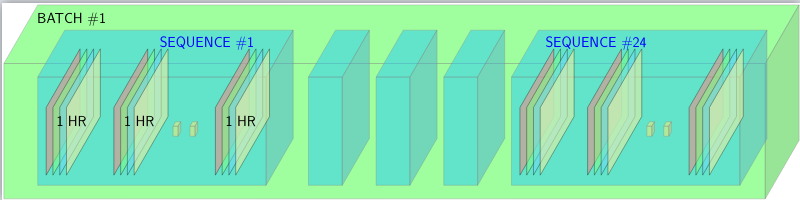
\includegraphics[scale=0.6]{ChapterX_Results_and_Conclusion/computational_experiments/temp_input_volume.png}
    \caption{Detailed sketch of the input volume to the $ConvLSTM-B_{10}-SL_{24}-32-3\times3-32-3 \times3$-model. Showing the content of the two first sequences in the first batch.}
    \label{fig:input_volume_conv_lstm}
\end{figure}

To test the importance of information in neigbouring pixels the model the $ConvLSTM-B_{10}-SL_{24}-32-1\times1-32-1 \times1$-model was trained and compared to the best model. %This is the architecture is the most similar \acrshort{ar}-models. 
As expected, this model has a higher loss than its sibling trained using a $3\times 3$. This is shown in Table \ref{tab:convlstmLoss} summarising the losses for all models in this study.
%you can see it has the worst Test loss among the trained models. This indicate that information from adjacent pixels is useful. Its necesarry to mention that there is a significant difference between a \acrshort{ar}-model and a \acrshort{convlstm}-model with $1\times 1$ kernel and that is that the \acrshort{ar}-model train a different weight in all pixels, while the \acrshort{convlstm}-model utilize the same weights over the entire grid. 
%Not suprising ths that the number of parameters increase as the kernel increasse. 
\clearpage

\subsection{GRID MAE}
This section contains the evaluation of the models against \acrshort{ecc}. The metric used is \acrshort{mae} and the period is 01.01.2014 to 31.12.2018. Figures \ref{fig:MAE_era}, \ref{fig:MAE_convlstm} and \ref{fig:MAE_AR} display the skill of the parameterization on the prediction of cloud cover in \acrshort{ecc}
Note the scales are different for each plot. Table \ref{tab:tot_mae_score} provide a summary of spatiotemporal skill of prediction of cloud cover. This shows that the overall best parameterization is made by the $AR-B-L5$-model. This is a bit misleading since its evaluated on its ability to predict one time step, which is a simpler task, than \acrshort{convlstm}-model, which is trained to predict 24 hours. 
\begin{table}[]
    \centering
    \begin{tabular}{cccc}
    \multicolumn{1}{c}{\textbf{}} & \textbf{ERA5} & \multicolumn{1}{c}{$\mathbf{AR-B-L_5}$} & \multicolumn{1}{c}{\textbf{$\mathbf{ConvLSTM-B_{10}-SL_{24}-32-3\times3-32-3\times3}$}} \\ \hline
    \textbf{MAE} & 0.20386 & 0.48502 &  0.33622 \\ \hline

    \end{tabular}
    \caption{\acrshort{mae} for the different cloud fractional cover parameterizations. }
    \label{tab:tot_mae_score}
\end{table}

%%%%%%%%%%%%%%%%%%%%%%%%%%%%%%%%%%%%%%% Commenting on spatial patterens
\begin{figure}
    \centering
    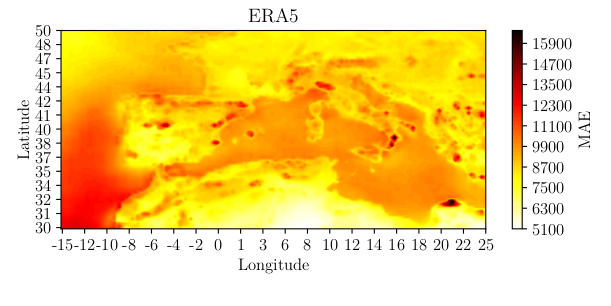
\includegraphics{python_figs/mae_era_vs_target_test_period_2014_to_2018.png}
    \caption{Evaluation of the parametrization in ERA5.}
    \label{fig:MAE_era}
\end{figure}

They all reveal regional biases. 

ERA5 
\textbf{A few examples on evaluation against observartions are used to highlight the}


It reveals systematic errors over the Mediterranean Sea and in the Atlantic Ocean of the coast of Gibraltar. Mountainous areas in the French and Italian Apls among other light up, revealing that they are predicted \textbf{skill er et bedre ord}. 

Figure \ref{fig:MAE_convlstm} show the performance of the best convolutional model in the period 2014-2018, the period is in fact a few hours shorter, since the models ran with ``drop remainder batch''. Both these representations of \acrshort{cfc} have trouble with the Nile Delta. This doesn't not seem to be the case for \textbf{update:the best ar model}.
\begin{figure}
    \centering
    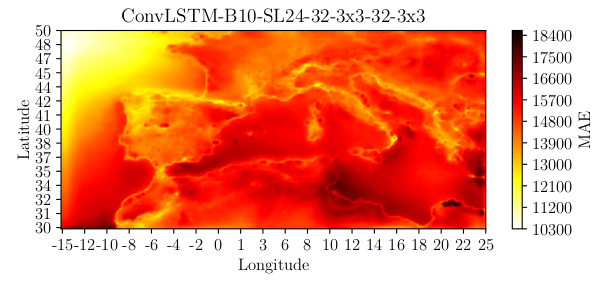
\includegraphics{python_figs/mae_convlstm_vs_target_test_period_2014_to_2018.png}
    \caption{Evaluation of the parameterization made by the $ConvLSTM-B_{10}-SL_{24}-32-3\times3-32-3 \times3$-model.}
    \label{fig:MAE_convlstm}
\end{figure}

\begin{figure}
    \centering
    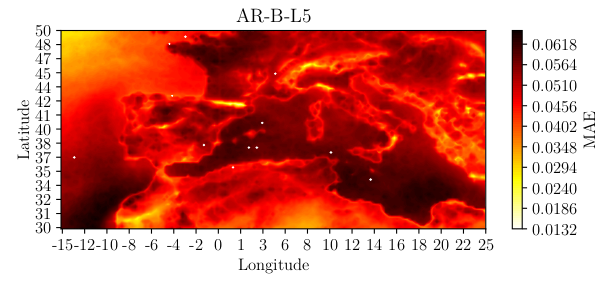
\includegraphics{python_figs/mea_best_ar_model_tcc_L5_in_folder_AR-B-L5.png}
    \caption{Evaluation of the parameterization made by the $AR-B-L_5$-model. The white dots visible is in total 12/13041 regression model having numerical issues related to non-invertable matrices.}
    \label{fig:MAE_AR}
\end{figure}

Half of this are caused by corrupt files.\textit{ We  did  not  recognize  before  later  in  the thesis  that  this  delimiting  layer  posed  a  problem  for  how  the  optimizer chose  the  pre-trained  model} This is not the case for all configurations as you can see in the other similar plots in the Appendix section \ref{app:mae_plots}. We therefore have reason to believe that this occured sometime during training. For the other pixel this remains an area of further investigation.

%%%%%%%%%%%%%%%%%%%%%%%%%%%%%%% Commenting on accumulated score 
Table \ref{tab:tot_mae_score} summarise the \acrshort{mae} over the entire domain. Keep in mind that these number are not directly comparable, ERA5 is assimilated, its a forecast rerun and bias corrected against observations. The \acrshort{convlstm}-model use the reanalysis data (environmental variables only) at each timestep to predict sequences of cloud cover. The ar model use the target at previous timesteps and reanalysis data 

Based in this the \acrshort{ar}-model goes out winning. One possible reason for this surprising result is that \acrshort{ar}-model is fitted against the \acrshort{ecc}, recall that 
the ERA5 is assimilated against a lot of observations, including radiance's from \acrlong{msg} \cite{ERA52020}.

All parameterizations reveal different systematic errors when compared to \acrshort{ecc}. Problematic regions for 

Summing over all pixels results in a MAE of $1.16508643\cdot10^8$. These systematic errors appear to be in region fewer observation, i.e. mountainous regions and over the sea. %Dust storm causing the red ocean off the coast of Sahara..?
%\begin{table}[]
    \centering
    \begin{tabular}{llll}
    \multicolumn{1}{c}{\textbf{}} & \textbf{ERA5} & \multicolumn{1}{c}{\textbf{AR}} & \multicolumn{1}{c}{\textbf{ConvLSTM}} \\ \hline
    MAE & $1.17\cdot10^8$ & $2.85\cdot10^7$ 2.85e+07 & $1.9 \cdot 10^8$ 
    \end{tabular}
    \caption{Total \acrfull{mae} in the period ... \textbf{Beregne disse som gjennomsnitt, hadde bare misforstått noe.}}
    \label{tab:tot_mae_score}
\end{table}

Med reanalyse som input for tidligere tidssteg gjør ar-modellene det veldig bra. However når det gjelder å predikere en hel sekvens går prestasjonen rask nedover. \textbf{Her vil det være mest riktig å predikere samme 24timers sekvenser for å sammenligne med ConvLSTM.} ERA5 er fremdeles assimilert 


\textbf{Flyttet fra AR kapitell. Figure \ref{fig:grid_mse_best_model} show the score of each pixel in the best model, \textbf{name best model}. This model got a remarkable performance, despite the fact that there is no information change among neighbouring pixels. The patteren in figure, show clear distinction between land and ocean, most likely i. The areas of the coast of Africa, Mediterranean ocean and the
The mountains areas light up as easier to predict. \textbf{Check if these are on average more cloudy.}}

\subsection{24-hour Cloud Cover Forecast}
\textbf{For the sequence plot of AR- it becomes clear that it has overfitted to the cloud cover at the previos timestep, this is not to surprising, makes dampend copies of the cloud cover until it becomes clear. Comment the score on the equivilent model is 10 times higher for TR.}

$AR-B-L_5$ $ConvLSTM-B_{10}-SL_{24}-32-3\times3-32-3 \times3$
In this section provide a visual comparison of the $AR-B-S-L5$-model, $ConvLSTM-B_{10}-SL_{24}-32-3\times3-32-3 \times3$-model, ERA5 and the target, \acrshort{cfc} in \acrshort{ECC}. Figure \ref{fig:pred_sequence} shows the first six hours of the evolution of the cloud cover forecast for the different models. This if the first plot in a series of four, showing the entire 24 hour forecast. The full series can be found in Appendix \ref{app:pred_sequence}. The series starts 2\textsuperscript{nd} January 2014.

The visual similarities of \acrshort{ecc}, \acrshort{ar}, and ERA5 is magnificent. At least for the first couple of hours. The AR model appear to be very sensitive to the initial conditions. The first hours seem to be a good match, for the next hour looks like the cloud cover retains the spatial patteren, but graually dissipate. Lets refer to this as the blurring effect from now on. At the end of the sequence the clouds are all located in the northern regions of the plot and the southern regions are clear. 

Both ERA5 and AR have softer transitions, between cloudy and cloud-free air than \acrshort{ecc}.

Like the statistical properties shown in Section X, the forecast provided \acrshort{convlstm} reveral the underlying surface. The outline of Europe is clearly visible. The forecast stick to the middle range cloud fraction values, starting with few cloud, with evolves toward a heavier overcast situation over Europe. 

Not surprising ERA5 is the most similar to \acrshort{ecc}, recall that this has the complex parameterization described in Section \ref{sec:era5_param}


%%%% TARGET PREDICITON ERA5
\begin{figure}[ht]
    \centering
    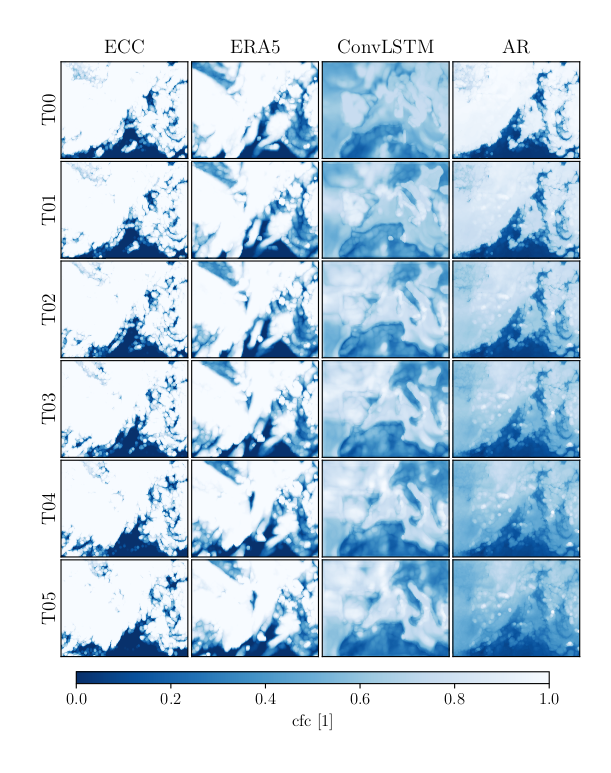
\includegraphics[sale=0.1]{python_figs/comparing_seq_part_1_of4_jan2.png}
    \caption{First of 4 part since the sequence is 24 hours long, the full series of plots for this sequence can be found in Appendix \ref{app:pred_sequence}.}
    \label{fig:pred_sequence}
\end{figure}
At first glance it clear that the \acrshort{convlstm}-model have learned which pixels are land and which is ocean. After a few hours its gets more distinct in its cloud cover and a weaker version of the triangle structure found in the three others begins to reveal itself. As the time pass by the cloud cover progress onto the continent and the \acrshort{convlstm} show signs of increased clod cover over parts of Spain and France.
The values are smoother and they are in this series are in the middle range.

\textbf{Comment on AR when its updated}
\textbf{sjekk appendix om det skjer noe som er ver å påpeke lenger ut i serien.}

The \acrshort{convlstm}-model is optimized to fit a sequence, while the \acrshort{ar}-model is optimized to fit the next timestep, not a sequence.
\textbf{Can you see this in Figure \ref{fig:target_predict_era5_horizontal} ..? Does the ar gradually become worse?}

\textbf{Run av med en oppsummerende setning om AR og ConvLSTM}
Is it evident that the \acrshort{convlstm} is better at predicting spatial patterns as expected or does it all resemble random noise. Is the predicted values in sample or out of sample.

The displayed sequence predicted by $ConvLSTM-B_{10}-SL_{24}-32-3\times3-32-3 \times3$-model contain no out of sample values. In total for the entire period of 2014-2018 $0.5\%$ is unphysical. The out-of-sample values predicted are purely on the negative sign, having a minimum at -1. 
%17140/3129840 = 0.005476318278250646

\textbf{Does AR ever predict out of sample values}
\textbf{Finn beste AR modell, prediker hele sekvensen, bergn MAE og tell ant. out of sample values}

Table \ref{tab:24hr_mae_score} shows the skill of the different models on predicting this 24 hours sequence. $ConvLSTM-B_{10}-SL_{24}-32-3\times3-32-3\times3$ rank highest having a score of 0.20386, ERA5 rank second with  $0.33622$ and $AR-B-L_5$ last with  $0.48502$. Note that a mean deviation of 0.46 is quite large when the data in question vary from 0 to 1. 
\begin{table}[]
    \centering
    \begin{tabular}{cccc}
    \multicolumn{1}{c}{\textbf{}} & \textbf{ERA5} & \multicolumn{1}{c}{$\mathbf{AR-B-L_5}$} & \multicolumn{1}{c}{\textbf{$\mathbf{ConvLSTM-B_{10}-SL_{24}-32-3\times3-32-3\times3}$}} \\ \hline
    \textbf{MAE} & 0.392 & 0.485 & 0.278 \\ \hline
    \textbf{MIN} & 0.0 & 0.004 & 0.0 \\ \hline
    \textbf{MAX} & 1.0 & 1.028 & 1.0 \\ 
    \end{tabular}
    \caption{\acrshort{mae}, minimum and maximum values for the 24-hour forecast period of 2\textsuperscrip{nd} January 2014. }
    \label{tab:24hr_mae_score}
\end{table}

The minimum value in this prediction (AR) is positive, and the maxmum is $1.028$. It a hundred and three percent cloudy. 

\textbf{Further west it is much drier, showers, turning a bit cooler, high temperatures for this time a year, heavy thundary dampours, }

\textbf{a short time ago}
\textbf{it continous to move across area one to 2}
\textbf{bringin terrential rain and damaging winds, and then it will move toward the }
\textbf{crashing into }
\textbf{grace the coast}
\textbf{The weather develops}
\subsection{Practical implications} \label{sec:practical_implications}
%It is necessary to have a understanding of the needs of the end product before conducting large machine learning projects. Answering questions like: What will it be used for and how can it be implemented in useful way?
A major downside of the data driven learning approach is the rigid resolution. A trained model can only be used on similar problems, with the same spatiotemporal resolution. For applications like climate models, output comes in a wide range of different resolutions. Before implementing the finished product in a new model of a different resolution, it would need to be retrained on the resolution of the climate model under development. This process involves both remapping of the dataset and retraining the model at the correct resolution. This is a time consuming process involving finding a new set of hyperparameters suitable for the new resolution. % It essentially means starting over.
%TS: Er ikke dette noe som bør undersøkes i fremtidige studier? M.a.o., er det alltid nødvendig "å starte om igjen" hvis oppløsningen endrer seg? Og hvor forskjellig må oppløsningen være for at det skal være nødvendig?

Once trained on global climate datasets, machine learning models provide fast results even for complex parameterization, which is what makes them suitable for the application of climate modelling. Most machine learning packages are developed using Python. \acrfull{esm} are increasingly also implemented in python. Methods for including the trained parameterizations need to be developed to further explore the potential of machine learning for climate modeling in the future.
%Uten transformasjon er det kanskje naturlig å sette prediksjoner < 0 til 0 og alle > 1 til 1. 
\textbf{There is an indication that from friday onwards, }

\textbf{The clouds streaming in from the south}
\textbf{Freahs weather, point out what the temperatures does in the week ahead}

\textbf{cloud cover across Europe and North Africa}
\textbf{somthing deveolp in cetral areas, quite active}

\textbf{First of all}

\subsection{Summary} \label{sec:summary_num}
In this section X antall modeller har blitt trent og evaluert på ecc. Nevn train test split?

Den best \acrshort{ar}-configuration is $AR-B-L_5$ \acrshort{mae} of $0.04901$. This is incrementally better than other $AR-B$-configurations by  varying on number of lags. Unfortunately, this model overfittet to the cloud cover at previous timesteps. Consequently its unable to produce sequences, it simply produce dampened copies of the initial cloud cover. The \acrshort{ar}-models might be to simple for performing this task? 

The best \acrshort{convlstm}-configuration was $ConvLSTM-B_{10}-SL_{24}-32-3\times3-32-3\times3$. Measured on MAE for the entire test period it performed rather badly, but it is was able to learn to predict a evolution in the cloud cover, unlike $AR-B-L_5$. The sequence predict cloud cover in the intermediate range of cloud fractions, resulting in a rather blurry image, it also reveal the geographical distribution underlying the data. 

Building a end-to-end trainables \acrshort{convlstm}-model. Managed to train a \acrshort{convlstm}-model on a larger dataset than other published studies.


and for the 24-hour sequence the mae was ok? 


This study has succesfully applied data driven learning to the cloud forcasting problem. 



On prediction a sequence, \acrshort{convlstm} improve further out in the sequence and \acrshort{ar}-model have a degraded performance.
\textit{The blurring effect, the pixels become more and more blurrered the further out in the sequence it progress}

\textit{The accuracy decrease as the prediction timestep goes on.}
% NOTES IN CASE I FORGET WHERE THE NUMBER CAME FROM
%\begin{enumerate}
%    \item Radar Echo: 1 sequence is 20 Frame one frame is 100x100. Train seq. 8148, 2037 for valid and 2037 for test. 
%    \item 1629600000 Num Train, 407400000 Num Valid and 407400000 num Test
%    \item KDD Weather data 21x31x5 365.25*24 (Train), 30*24(Valid, test)
%    \item 28513800 (Train) samples, 2343600 (Valid, Test)
%\end{enumerate}
%\textbf{Ønsker å understreke dette for det er }
It is more difficult to train a models on a larger amount of data. 
